%!TEX TS-program = xelatex

% Данный шаблон подготовлен для курса LaTeX в РАНХиГС
% на основе шаблона 
% Данилы Фёдоровых (danil@fedorovykh.ru),
%  который использовал его в курсе 
% <<Документы и презентации в \LaTeX>> НИУ ВШЭ
% Исходная версия шаблона --- 
% https://www.writelatex.com/coursera/latex/5.1


\documentclass[t, dvipsnames]{beamer}  % [t], [c], или [b] --- вертикальное выравнивание на слайдах (верх, центр, низ)
%\documentclass[handout, dvipsnames]{beamer} % Раздаточный материал (на слайдах всё сразу)
%\documentclass[aspectratio=169, dvipsnames]{beamer} % Соотношение сторон
\setbeamertemplate{navigation symbols}{}%remove navigation symbols

%\usetheme{Berkeley} % Тема оформленияLLL
%\usetheme{Bergen}
\usetheme{CambridgeUS}
%\usetheme{Boadilla}

\usecolortheme{crane} % Цветовая схема

%\useoutertheme{infolines} % Навигация 
%\useoutertheme{tree}
%\useoutertheme{miniframes}
%\useoutertheme{shadow}
%\useoutertheme{sidebar}
%\useoutertheme{smoothbars}
%\useoutertheme{smoothtree}
%\useoutertheme{split}
%\useoutertheme{default}


\useinnertheme{circles}
%\useinnertheme{rectangles}
%\useinnertheme{rounded}
%\useinnertheme{inmargin}


%%% Работа с русским языком
\usepackage[english,russian]{babel}   %% загружает пакет многоязыковой вёрстки
\usepackage{fontspec}      %% подготавливает загрузку шрифтов Open Type, True Type и др.
\defaultfontfeatures{Ligatures={TeX},Renderer=Basic}  %% свойства шрифтов по умолчанию
\setmainfont[Ligatures={TeX,Historic}]{Times New Roman} %% задаёт основной шрифт документа
\setsansfont{Arial}                    %% задаёт шрифт без засечек
\setmonofont{Courier New}
\usepackage{indentfirst}
\frenchspacing

%% Beamer по-русски
\newtheorem{rtheorem}{Теорема}
\newtheorem{rproof}{Доказательство}
\newtheorem{rexample}{Пример}

%%% Дополнительная работа с математикой
\usepackage{amsmath,amsfonts,amssymb,amsthm,mathtools} % AMS
\usepackage{icomma} % "Умная" запятая: $0,2$ --- число, $0, 2$ --- перечисление

%% Номера формул
%\mathtoolsset{showonlyrefs=true} % Показывать номера только у тех формул, на которые есть \eqref{} в тексте.
%\usepackage{leqno} % Нумерация формул слева

%% Свои команды
\DeclareMathOperator{\sgn}{\mathop{sgn}}

%% Перенос знаков в формулах (по Львовскому)
\newcommand*{\hm}[1]{#1\nobreak\discretionary{}
{\hbox{$\mathsurround=0pt #1$}}{}}

%%% Работа с картинками
\usepackage{graphicx}  % Для вставки рисунков
\graphicspath{{images/}{images2/}}  % папки с картинками
\setlength\fboxsep{3pt} % Отступ рамки \fbox{} от рисунка
\setlength\fboxrule{1pt} % Толщина линий рамки \fbox{}
\usepackage{wrapfig} % Обтекание рисунков текстом

%%% Работа с таблицами
\usepackage{array,tabularx,tabulary,booktabs} % Дополнительная работа с таблицами
\usepackage{longtable}  % Длинные таблицы
\usepackage{multirow} % Слияние строк в таблице

%%% Программирование
\usepackage{etoolbox} % логические операторы

%%% Другие пакеты
\usepackage{lastpage} % Узнать, сколько всего страниц в документе.
\usepackage{soul} % Модификаторы начертания
\usepackage{csquotes} % Еще инструменты для ссылок
\usepackage{multicol} % Несколько колонок


\usepackage{hyperref}
\usepackage{xcolor}
\hypersetup{        % Гиперссылки
    unicode=true,           % русские буквы в раздела PDF
    pdftitle={Заголовок},   % Заголовок
    pdfauthor={Автор},      % Автор
    pdfsubject={Тема},      % Тема
    pdfcreator={Создатель}, % Создатель
    pdfproducer={Производитель}, % Производитель
    pdfkeywords={keyword1} {key2} {key3}, % Ключевые слова
    colorlinks=true,        % false: ссылки в рамках; true: цветные ссылки
    linkcolor=,          % внутренние ссылки
    citecolor=green,        % на библиографию
    filecolor=magenta,      % на файлы
    urlcolor=blue           % на URL
} 

%fffff3
\definecolor{backgr}{HTML}{fffff3}
\setbeamercolor{normal text}{fg=black,bg=backgr}
%\setbeamercolor{frametitle}{fg=blackbg=backgr}
%\setbeamercolor{normal text}{bg=yellow}
%\setbeamercolor{section in toc}{fg=yellow}
%\setbeamercolor{subsection in toc}{fg=blue}
%\setbeamercolor{frametitle}{fg=darkblue}
% How to change colour of Navigation Bar in Beamer -  много интересного

%Пример команд, задающих внешний вид блока
\setbeamercolor{block title}{fg=white,bg=MidnightBlue}
\setbeamerfont{block title}{family=\sffamily}
\setbeamercolor{block body}{bg=white}
\setbeamertemplate{blocks}[rounded][shadow=true]

\title[Короткое название]{Длинное название вашей презентации \\ в несколько строчек }
\subtitle{Подзаголовок презентации / Название конференции}

\author[Имя автора]{Имя автора \\ \smallskip \scriptsize \href{mailto:author@ranepa.ru}{\nolinkurl{author@ranepa.ru} } \\ \smallskip \url{http://ranepa.ru}}

%\author[Имя автора]{Имя автора \\ \smallskip \scriptsize \href{mailto:author@ranepa.ru}{author@ranepa.ru} \\ \smallskip  \href{http://ranepa.ru}{http://ranepa.ru} }

\institute[РАНХиГС]{
  Российская Академия Народного Хозяйства и  \\ Государственной Службы при Президенте Российской Федерации}
\date[Короткая дата]{\today}
%\logo{
\includegraphics[height=0.8cm]{zHFFO}}
\logo{{\color{black} \Huge{\LaTeX}}}
\titlegraphic{
\includegraphics[height=0.8cm]{zHFFO}}
%\titlegraphic{Научный руководитель: Фамилия Имя}




\begin{document}

\frame[plain]{\titlepage}	% Титульный слайд

\frame[plain]{\tableofcontents}

\section{Поочередное появление объектов}
\subsection{Команда pause}
 
\begin{frame}
	\frametitle{\insertsection} 
	\framesubtitle{\insertsubsection}
	\begin{itemize}
		\item beamer ---  это \alert{удобный} \textbf{пакет} для создания презентаций.
		\item Это наш первый слайд \pause
		\item Вот \href{http://ctan.uni-altai.ru/macros/latex/contrib/beamer/doc/beameruserguide.pdf}{полное руководство по beamer}
		\pause
		\item Паузу можно поставить в любом \pause месте.
		\item Для печати презентации есть режим handout.
	\end{itemize}
\end{frame}

\subsection{Более сложно}

%\begin{frame}
%	\frametitle{Поочередное появление пунктов списка}
%	\framesubtitle{\insertsubsection}
%    \uncover<4-6>{Эта строчка появляется не сразу, но занимает место.}
%    \only<5-7>{Эта строчка появляется не сразу и не занимает места.}
%    \begin{enumerate}
%        \item<1-5> Сначала появляются первый и последний пункт (первый потом исчезнет).
%        \item<2-> Потом второй
%        \item<3-> И наконец третий
%        \item<1-> Последний пункт появляется вместе с первым
%    	\item<6-> В самом конце первый пункт исчезает, зато появляется картинка: \insertlogo.
%    \end{enumerate}
%    \alt<4>{Это \alert{четвертый} слайд}{Это не четвертый слайд.}
%    \temporal<3-4>{Слайды 1, 2}{Слайды 3, 4}{Сайды 5, 6, 7, ...}
%\end{frame}

\begin{frame}{Пример из руководства}
    \uncover<4->{Эта строчка появляется не сразу, но занимает место.}
    \only<5->{Эта строчка появляется не сразу и не занимает места.}
\begin{enumerate}
   \item  \textbf{This line is bold on all three slides.}
    \item \textbf<2>{This line is bold only on the second slide.}
   \item  \textbf<3>{\alert<4>{This line is bold only on the third slide.}}
   \item \textbf<3,4>{Эта строчка жирная на 3-м и 4-м слайде.}
	 \item \color<3-4>[RGB]{255,0,0} Этот текст красный только на сладах 3-4.
    \end{enumerate}
        \alt<4>{Это \alert{четвертый} слайд}{Это не четвертый слайд.} \\
    \temporal<3-4>{Слайды 1, 2}{Слайды 3, 4}{Сайды 5, 6, 7, ...}
\end{frame}

\subsection*{АЛЛО КЛАССНЫЕ ПАРНИ КОЛЬ ПРО ДРУГИХ ФАКТЫ ВЫСТАВЛЯЕТЕ ЖДЕМ ТЕПЕРЬ ВАШИ}
\begin{frame}[shrink=5]
	\frametitle{Поочередное появление пунктов списка}
	\framesubtitle{\insertsubsection}
     \begin{enumerate}
        \item<1-> \alert<3-5>{Единственный дипломированный преподаватель LaTeX}
        \item<2-> Проверяет дз своего научного руководителя (не всегда)
        \item<3-> Первый раз ведет лекцию перед студентами
      \only<10->{ \item Надеется не делать д/з как минимум 7 лет}
    	\item<4-> \color<4-5>[RGB]{255,0,0} {Любит Чёрный супрематический квадрат Малевича}
    	\item<5-> Заказал московский снег в одном московском ресторане 
    	\item<6-> \textbf<3>{Очень любит наклеечки на мак}
    	\item<7-> Так же как и свой мак
    	\item<8-> Участвовал в рыцарском турнире (и не одном)
    	\item<9-> Делаю презентации только в \insertlogo
    \end{enumerate}
\end{frame}
\section{Об оформлении}
\subsection{Презентация в целом}

\begin{frame}[c] % [t], [c], или [b] --- вертикальное выравнивание на слайде (верх, центр, низ)
	\frametitle{\insertsection}
	\framesubtitle{\insertsubsection}
	\begin{itemize}
			\item Варианты оформления можно посмотреть здесь:  \href{http://www.hartwork.org/beamer-theme-matrix/}{http://www.hartwork.org/beamer-theme-matrix/} 
			\item Есть и другие сайты с примерно одинаковым функционалом:
					\begin{itemize}
					\item \href{https://mpetroff.net/files/beamer-theme-matrix/}{https://mpetroff.net/files/beamer-theme-matrix/}
					\item \href{http://deic.uab.es/~iblanes/beamer_gallery/}{http://deic.uab.es/~iblanes/beamer\_gallery/}
				\end{itemize}
		\item Можно создавать свои темы. 
		\item Можно выровнять текст на слайдах по верхнему краю с использованием опции [t] (у всей презентации ---  \texttt{[t]{beamer}} или у отдельного слайда \texttt{{frame}[t]}) 
		\item Можно регулировать формат слайдов с помощью опции \texttt{[aspectratio=xx]}. Например, \texttt{[aspectratio=169]}. 
	\end{itemize}
\end{frame}

\subsection{На слайде}

\begin{frame}
	\frametitle{\insertsection}
	\framesubtitle{\insertsubsection}
    \begin{block}{Первый блок}
		Текст первого блока
	\end{block}
	\begin{block}{Второй блок}
		Текст второго блока
    \end{block}
	\begin{block}{Кнопка}
		\hyperlink{lab}{\beamerbutton{Кнопка со ссылкой}} 
	\end{block}
\end{frame}

\begin{frame}
	\frametitle{\insertsection}
	\framesubtitle{\insertsubsection}
    \begin{rtheorem}
		Формулировка теоремы.    
	\end{rtheorem}
	\begin{rproof}
		Текст доказательства.
    \end{rproof}
	\begin{rexample}
		Текст примера.
	\end{rexample}
\end{frame}

\section{Формулы}

\begin{frame}
	\frametitle{\insertsection}
	\begin{itemize}
		\item $\displaystyle\int_0^1 x=1/2$  
		\item $2\times 2=4$, $2^2=4$ 
		\item $\displaystyle\frac{5}{\alert{6}}=\frac{1}{1+\frac{1}{5}}$ 
	\end{itemize}
	\begin{equation}
	Y=K^\alpha \times L^{1-\alpha}
	\end{equation}
\end{frame}




\section{Большой текст}

\begin{frame}[shrink=7]\label{lab}  % Опцию shrink лучше не использовать
	\frametitle{\insertsection}
	
	\textsl{Чуден Днепр при тихой погоде, когда вольно и плавно мчит сквозь леса и горы полные воды свои. Ни зашелохнет; ни прогремит. Глядишь, и не знаешь, идет или не идет его величавая ширина, и чудится, будто весь вылит он из стекла, и будто голубая зеркальная дорога, без меры в ширину, без конца в длину, реет и вьется по зеленому миру. Любо тогда и жаркому солнцу оглядеться с вышины и погрузить лучи в холод стеклянных вод и прибережным лесам ярко отсветиться в водах. Зеленокудрые! они толпятся вместе с полевыми цветами к водам и, наклонившись, глядят в них и не наглядятся, и не налюбуются светлым  своим зраком, и усмехаются к нему, и приветствуют его, кивая ветвями. В середину же Днепра они не смеют глянуть: никто, кроме солнца и голубого неба, не глядит в него. Редкая птица долетит до середины Днепра. Пышный! ему нет равной реки в мире. Чуден Днепр и при теплой летней ночи, когда все засыпает --- и человек, и зверь, и птица; а бог один величаво озирает небо и землю и величаво сотрясает ризу.}

	\hfill{\textit{Н. В. Гоголь}}
\end{frame} 


{
\usebackgroundtemplate{ 
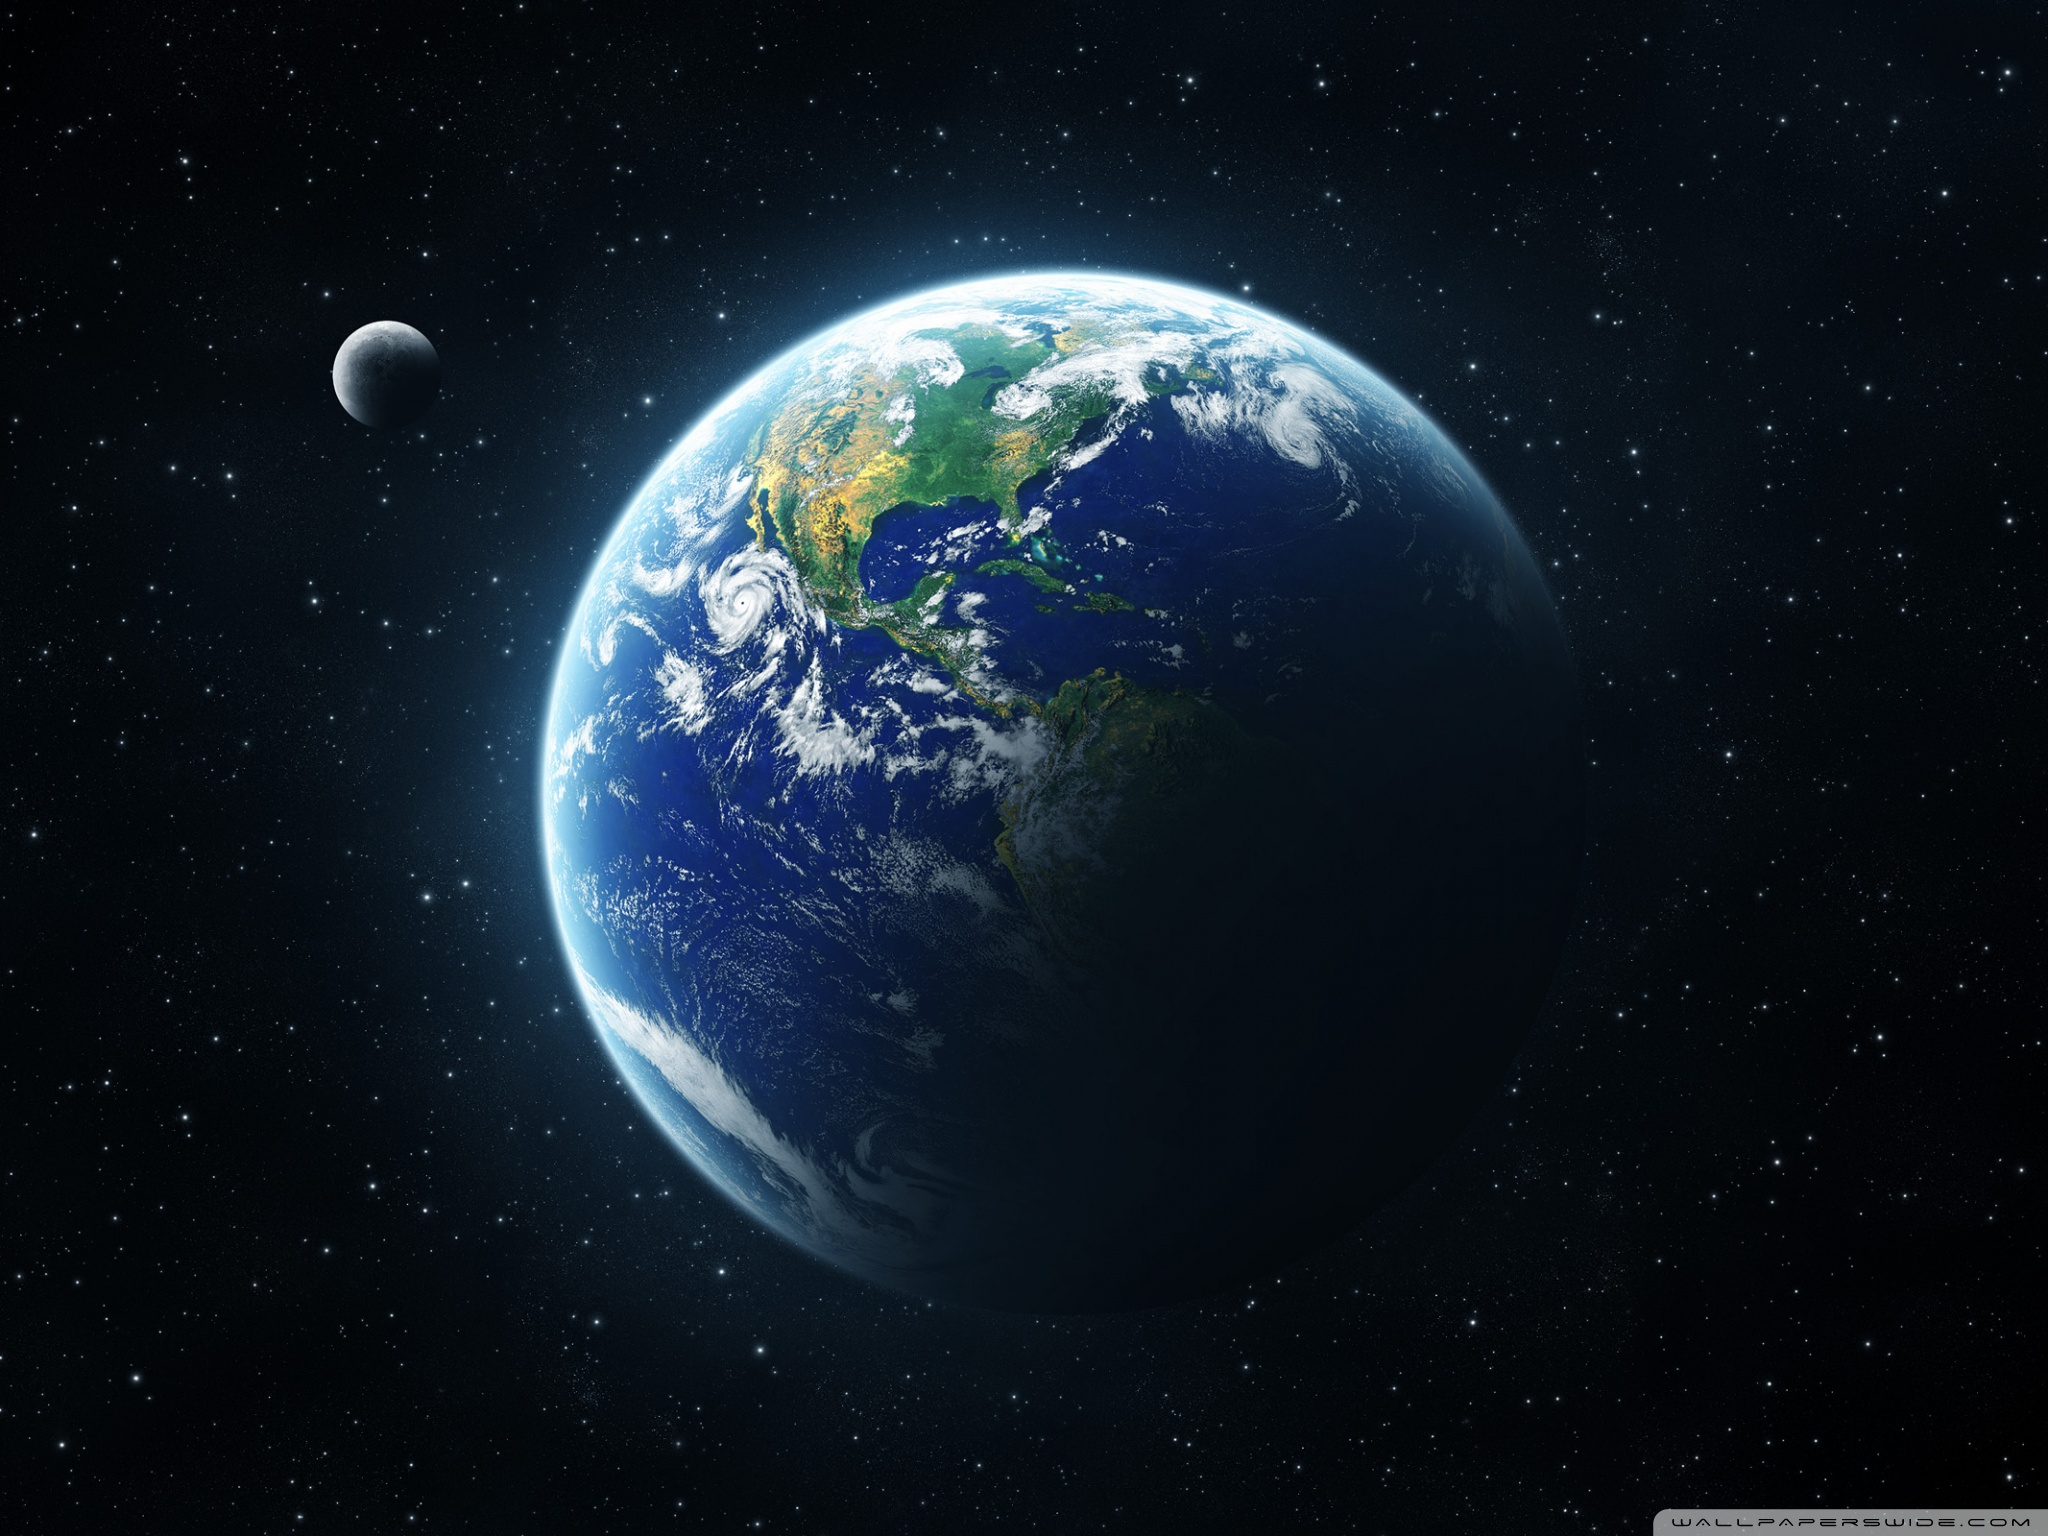
\includegraphics[width=\paperwidth]{earth-from-space-1} }
\begin{frame}
\color{white}Чуден Днепр при тихой погоде, когда вольно и плавно мчит сквозь леса и горы полные воды свои. Ни зашелохнет; ни прогремит. Глядишь, и не знаешь, идет или не идет его величавая ширина, и чудится, будто весь вылит он из стекла, и будто голубая зеркальная дорога, без меры в ширину, без конца в длину, реет и вьется по зеленому миру. Любо тогда и жаркому солнцу оглядеться с вышины и погрузить лучи в холод стеклянных вод и прибережным лесам ярко
\end{frame}
}
 
\includeonlylecture{} % Можно поместить это в преамбулу

\lecture{Лекция 1}{lec1}
	\section{<<Лекции>>}
	\begin{frame}
		\frametitle{\insertsection}
		lecture-функционал позволяет включать в презентацию только отдельные слайды, а в одном файле держать целый цикл презентаций 
	\end{frame}

\lecture{Лекция 2}{lec2}
	\section{Это лекция 2}
	\begin{frame}
	\frametitle{\insertsection}
		Все frames не внутри какой-нибудь lecture присутствуют всегда. Если нет  команды \verb"includeonlylecture{}", то все лекции тоже присутствуют всегда. Отдельную лекцию можно показать с помощью \verb"includeonlylecture{}".
	\end{frame}


\lecture{ДЗ}{HW}	
\section{ДЗ в beamer}

\begin{frame}[shrink=20]
	\frametitle{\insertsection}	
Сделайте презентацию, которая могла бы сопровождать ваш доклад на научном семинаре по теме вашего НИРа. В презентации должно быть отражено
\begin{itemize}
	\item[1] Презентация содержит титульный слайд с вашем именем, названием работы и прочей информацией. 
	\item[1] Должно быть оглавление сразу после титульного слайда 
	\item[1] Презентация содержит как \verb"section", так и \verb"subsection" (возможно не везде)
	\item[1] На каждом сайде перед названием \verb"section" должен быть номер, также и с \verb"subsection" и при изменении номера меняются автоматически  
	\item[2] Создайте новое окружение (вместе \verb"frame"), в котором будет автоматически подставляться заголовок и подзаголовок (c \verb"etoolbox" бонус)
	\item[1] Перед началом нового раздела (\verb"section") должно отображаться оглавление с подсвеченным разделом, который начинается на следующем слайде. 
	\item[2] Дополнительно, если предыдущий пункт выполняется автоматически при создании нового раздела 
	\item[1+1] Презентация должна содержать таблицы и картинки (должно быть понятно что именно отображена на картинках и на графиках) 
	\item[1] Причем на некоторых слайдах картинки должны появляться постепенно
	\item[1] Строки в таблице также должны появляться постепенно
	\item[1] Какая-то информация на слайде должна исчезать после нескольких переходов 
	\item[1] Соблюдайте общие правила оформления презентаций к семинарам 	
	\item[$\infty$] Использовать корпоративные цвета РАНХиГС, логотипы и т.\:д. согласно официальному брендбуку Академии
	\end{itemize}
\end{frame}



\begin{frame}[plain]
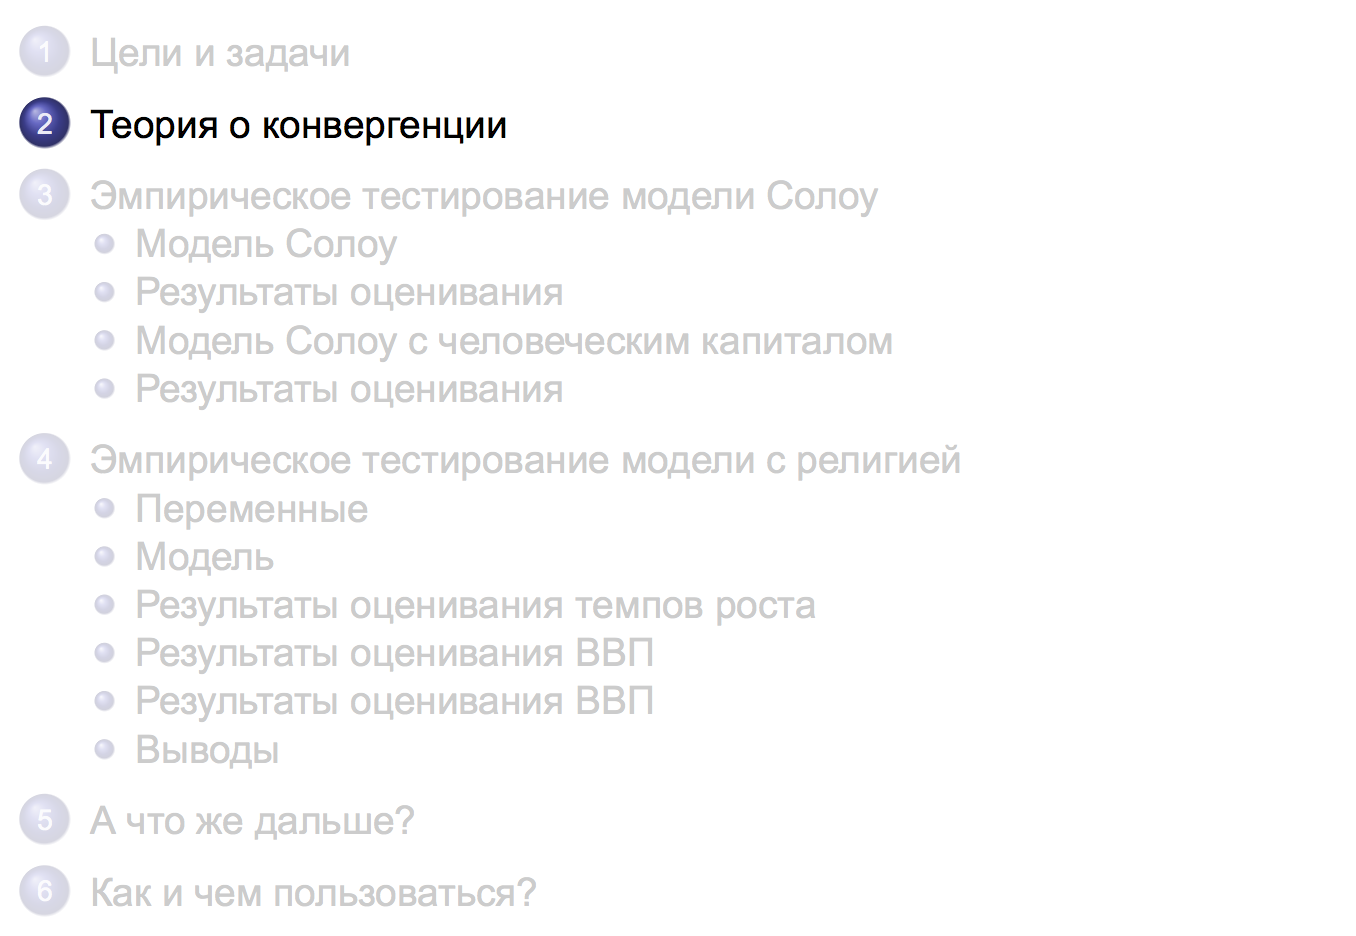
\includegraphics[width=\paperwidth]{hw} 
\end{frame}

\end{document}